%%%%%%%%%%%%%%%%%%%%%%%%%%%%%%%%%%%%%%%%%%%%%%%%%%%%%%%%%%%%%
%% Begin exercise %%
%%%%%%%%%%%%%%%%%%%%%%%%%%%%%%%%%%%%%%%%%%%%%%%%%%%%%%%%%%%%%
\ex{Rectifiers}

%%%%%%%%%%%%%%%%%%%%%%%%%%%%%%%%%%%%%%%%%%%%%%%%%%%%%%%%%%%%%
%% Task 1: B2U topology with capactive filtering %%
%%%%%%%%%%%%%%%%%%%%%%%%%%%%%%%%%%%%%%%%%%%%%%%%%%%%%%%%%%%%%
\task{B2U topology with capactive filtering}
An uncontrolled single-phase, two-pulse rectifier circuit with capacitive filtering 
is shown in \autoref{fig:B2U_Topology_Cap_Filtering}.
All components, including the diodes, are assumed to be ideal. On the input side, 
the single-phase AC supply with voltage $u$ is connected, while on the output side, 
a smoothing capacitor $C$ and a constant current load $I_\mathrm{L}$ are present.

%%%%%%%%%%%%%%%%%%%%%%%%%%%%%%%%%%%%%%%%%%%%%%%%%%%%%%%%%%%%%%%%%%%%%%%
 % B2U rectifier with capacitive output filtering
%%%%%%%%%%%%%%%%%%%%%%%%%%%%%%%%%%%%%%%%%%%%%%%%%%%%%%%%%%%%%%%%%%%%%%%
    \begin{figure}[htb]
        \begin{center}
            \begin{circuitikz}[european currents,european resistors,american inductors]
                \draw
                % Base point for voltage supply
                (0,0) coordinate (jU1v)
                % Add supply U1 [open, o-o, v = $u_1(t)\hspace{0.5cm}$, voltage = straight]
                (jU1v) to [open, o-o, v = $u_1(t)\hspace{0.5cm}$, voltage = straight] ++(0,-2) coordinate (jU1g)
                % Add arrow and Text
                (jU1v) ++(0.5,0) node[currarrow](I1){}  
                (I1)  node[anchor=south,color=black]{$i_\mathrm{1}(t)$}  
                % Add connection to diode D1/D4
                (jU1v) to [short, -*] ++(2,0) coordinate (jaD1)
                % Add D1 
                (jaD1) to [diode, l=$D_1$]  ++(0,1.5)  coordinate (jkD1)
                % Add D4 connection S
                (jaD1)  ++(0,-3.5)  coordinate (jaD4)
                % Add D4 
                (jaD4) to [diode, l=$D_4$] ++(0,1.5)  coordinate (jkD4)
                % Add connection D4 to D1
                (jkD4) to [short, -]  (jaD1)
                % Add connection to diode D3/D2
                (jU1g) to [crossing, -*, mirror] ++(4,0)  coordinate (jkD2)
                % Add connection D2 to D3
                (jkD2) to [short, -] ++(0,2) coordinate (jaD3)
                % Add D3 
                (jaD3) to [diode, l=$D_3$]  ++(0,1.5)  coordinate (jkD3)
                % Add D2 connection 
                (jkD2)  ++(0,-1.5)  coordinate (jaD2)
                % Add D2 
                (jaD2) to [diode, l=$D_2$] (jkD2)
                % Add connection D1 to D3
                (jkD1) to [short, -*] (jkD3)                
                % Add connection to capacitor plus
                (jkD3) to [short, -*, i=$i_2(t)$] ++(2,0) coordinate (jvCp)
                % Add connection to current source vI0
                (jvCp) to [short, -] ++(1.5,0) coordinate (jvI0)
                % Add coordinate of current source gI0
                (jvI0) ++(0,-5) coordinate (jgI0)
                % Add current source I0
                (jvI0) to [isource, l=$I_0$] (jgI0)
                % Add connection to capacitor minus
                (jgI0) to [short, -*] ++(-1.5,0) coordinate (jgCm)
                % Add capacitor
                (jvCp) to [C, v= $u_\mathrm{2}(t)$, voltage = straight, l=$C$, i=${i_\mathrm{C}(t)}$] (jgCm)
                % Add connection to D2
                (jgCm) to [short, -*] (jaD2)
                % Add connection D2 to D4
                (jaD2) to [short, -] (jaD4);
            \end{circuitikz}
    \end{center}
        \caption{B2U rectifier with capacitive output filtering.}
        \label{fig:B2U_Topology_Cap_Filtering}
    \end{figure}




The angle $\alpha_\mathrm{1}$ represents the point in time at which two of the four diodes begin to conduct, 
i.e., when the capacitor is recharged from the mains supply. From the angle $\alpha_\mathrm{2}$
all four diodes are blocked, meaning the capacitor discharges through the load. 
A steady-state operation is assumed for this task.

\subtask{Calculate the two angles $\alpha_1$ and $\alpha_2$.
Note: It is more convenient to calculate $\alpha_2$ first. For the calculation of $\alpha_1$  
you can use the following simple approximation: $sin(x) = x$. 
(This approximation is sufficiently accurate within a range of approximately $\SI{25}{\degree}$  around the zero point of the sine function.)}
\vspace{2em}\par
If you were unable to solve task (a), please use $\alpha_1=\SI{19.3}{\degree}$ and $\alpha_2=\SI{112.8}{\degree}$.

\subtask{Sketch the waveform of the capacitor voltage $u_\mathrm{C}$ for the angles $\alpha_\mathrm{1}$ and $\alpha_\mathrm{2}$ calculated in previous subtask.}

\subtask{Sketch the time-dependent waveform of the current $i_\mathrm{1}(t)$  and $i_\mathrm{2}(t)$.}

\subtask{Assume the smoothing capacitor is very large, i.e., $C\rightarrow \infty$ .What is the average active power $P_\mathrm{L}$ 
absorbed by the current source? What will $P_\mathrm{L}$ be if $C=\SI{330}{\milli\ampere}$?}


\subtask{What is the minimum blocking voltage ratings of the diodes to ensure that the rectifiers is not damaged?}



%%%%%%%%%%%%%%%%%%%%%%%%%%%%%%%%%%%%%%%%%%%%%%%%%%%%%%%%%%%%%
%% Task 2: PFC rectifier %%
%%%%%%%%%%%%%%%%%%%%%%%%%%%%%%%%%%%%%%%%%%%%%%%%%%%%%%%%%%%%%
\task{PFC rectifier}
Due to the constantly increasing load on the grid with harmonics as a result of the use of power converters, the regulations regarding the permissible harmonic content of the current consumption of electrical consumers are being tightened. It is therefore necessary, e.g. for the rectification of single-phase AC mains voltage, for example, it is necessary to design power converters with a high power factor or a largely sinusoidal input current. 
A variant of a PFC rectifier circuit is shown in \autoref{fig:Boost converter with single-phase diode bridge_topology}. The system consists of a diode bridge $(D_{\mathrm{1}} \, \dots \, D_{\mathrm{4}})$, an inductor $L$, a power transistor $T$ (usually a power MOSFET), a freewheeling diode $D_\mathrm{5}$ and an output capacitor $C$. The prerequisite for the use of the boost converter is: $u_\mathrm{d} = U_\mathrm{d}>U_\mathrm{1}$. The boost converter is operated with a modified current control method ('Average Current Mode Control') for which the switching frequency $f_\mathrm{T}$ has a constant value $f_\mathrm{T} = \SI{20}{\kilo\hertz}$. This is realized by comparing the current controller output variable with a triangular oscillation with switching frequency $f_\mathrm{T} = \SI{20}{\kilo\hertz}$ and suitable amplitude is compared. Let $L = \SI{570}{\micro\henry}$ and the inductance carry a continuous current. Definition: Transmission ratio: $M = \frac{ U_\mathrm{d}}{\hat U_\mathrm{1}}$
%%%%%%%%%%%%%%%%%%%%%%%%%%%%%%%%%%%%%%%%%%%%%%%%%%%%%%%%%%%%%%%%%%%%%%%
 % Boost converter with single-phase diode bridge Schematic
%%%%%%%%%%%%%%%%%%%%%%%%%%%%%%%%%%%%%%%%%%%%%%%%%%%%%%%%%%%%%%%%%%%%%%%
    \begin{figure}[htb]
        \begin{center}
            \begin{circuitikz}[european currents,european resistors,american inductors]
         % Input rectifier
         \draw (0,0) to [open, o-o, v = $u_1(t)\hspace{0.5cm}$, voltage = straight] ++(0,-2) coordinate (A)
         (0,0) to [short, i>^=$i_1(t)$] ++(0.75,0) to [short, -*] ++(0.75,0)
         to [diode, l=$D_1$]  ++(0,1.5)
         to [short, -*] ++(1.5,0) coordinate (C)
         to [diode, l=$D_3$, invert]  ++(0,-1.5)
         to [short] ++(0, -2) coordinate (B)
         to [diode, l=$D_2$, invert, -*]  ++(0, -1.5) coordinate (D)
         to [short] ++(-1.5,0)
         to [diode, l=$D_4$]  ++(0, 1.5)
         to [short] ++(0, 2)
         (B) to [short, *-]++(-0.5,0) to [crossing, mirror] ++(-2,0)
         to [short] (A);

         % DC/DC converter
         \draw node[fourport, circuitikz/quadpoles/fourport/width=2.25, circuitikz/quadpoles/fourport/height=2.8] (DCDC) at (7.75,-1) {DC/DC}; 
         \draw (C) to [short] ++(1.5,0) coordinate (G)
         to [short] (DCDC.port4 -| G) 
         to [short,-*] ++(0.5,0) coordinate (voltin)
         to [short, i=$i'(t)$] (DCDC.port4)
         (D) to [short] ++(1.5,0) coordinate (H)
         to [short] (DCDC.port1 -| H) -- ++(0.5,0)
         to [currtap, name=ct1] (DCDC.port1)
         (DCDC.port4 -| G) to [open,v = $u'(t)\hspace{0.5cm}$, voltage = straight] (DCDC.port1 -| G);

         % Inner part
         \draw (DCDC.port4) to [L, l=$L$] ++(1.75,0) coordinate (boostup)
         to [diode, l=$D_5$] (DCDC.port3)
         (boostup) to [Tnpn, n=npn, invert,*-*, l=$\hspace{0.5cm}T$] (DCDC.port2 -| boostup)
         (DCDC.port2) -- (DCDC.port1); 


         % Output filter and load
         \draw (DCDC.port3) to [short, i=$i_2(t)$] ++(0.9,0) coordinate (I)
         to [short] (C -| I)
         to [short] ++(1,0) coordinate (E)
         to [short] ++(0,-1.5)
         to [C, v= $u_2(t)$, voltage = straight, l=$C$, i=${i_\mathrm{C}(t)}$] ++(0,-2)
         to [short] ++(0,-1.5) coordinate (F)
         to [short] (D -| I)
         to [short] (DCDC.port2 -| I) -- (DCDC.port2)
         (E) to [short, *-*] ++(1.25,0) coordinate (currout) -- ++(0.75,0)
         to [short] ++(0,-1.5)
         to [R,  l=$R$, i=${i_\mathrm{R}(t)}$] ++(0,-2)
         to [short] ++(0,-1.5)
          to [short, -*] (F);

         % Controller
         \draw let \p1 = (DCDC.south) in node[draw, minimum width=1.2cm, minimum height=0.9cm] (ctrl) at (\x1,-4.1) {Controller};
         \coordinate (ctrl1) at ($(ctrl.north west)!.5!(ctrl.west)$);
         \coordinate (ctrl2) at ($(ctrl.south west)!.5!(ctrl.west)$);
         \draw[dashed] (ctrl.north) -- (DCDC.south) node[midway, right] {$d(t)$} -- ++(0,0.5) coordinate (ctrl3)
         to [short] (ctrl3 -| npn.B) -- (npn.B);
         \draw[->, dashed] (ct1.tap) -- (ctrl1 -| ct1.tap) -- (ctrl1) node[right, above, anchor = south east] {$i'(t)$};
         \draw[->, dashed] (voltin) -- (ctrl2 -| voltin) -- (ctrl2) node[right, below, anchor = north east] {$u'(t)$};
         \draw[->, dashed] (currout) -- (ctrl.east -| currout) -- (ctrl.east) node[left, above, anchor = south west] {$u_2(t)$};
        \end{circuitikz}
    \end{center}
        \caption{PFC rectifier with single-phase diode bridge and a cascaded DC/DC boost converter.}
        \label{fig:Boost converter with single-phase diode bridge_topology}
    \end{figure}


\begin{table}[ht]
    \centering  % Zentriert die Tabelle
    \begin{tabular}{llll}
        \toprule
        
        Input voltage: &  $u_{\mathrm{1}}(t) = \hat U_{\mathrm{1}} \sin(\omega t) = \sqrt{2} \cdot \SI{230}{\volt} \sin(\omega t)$ & Output voltage: & $u_{\mathrm{2}}(t) = \SI{400}{\volt}$ \\ 
        Output power: & $P_\mathrm{2} = \SI{4}{\kilo\watt}$  & Circular frequency: & $\omega = 2 \pi \SI{50}{\hertz}$ \\ 
        Inductance: & $L = \SI{570}{\micro\henry}$
         & switching frequency: & $f_\mathrm{T} = \SI{20}{\kilo\hertz}$\\
        \bottomrule
    \end{tabular}
    \caption{Parameters of the PFC rectifier.}  
    \label{table:ex05_Parameters of the circuit}
\end{table}

\subtask{Specify the voltage transformation ratio $m(t)= \frac{u_{\mathrm{2}}(t)}{u'(t)}$ as a function of the duty cycle $D(t)$ is specified.}
\begin{solutionblock}
    
    \begin{equation}
        U_{\mathrm{L}} = d(t) u'(t) + (1-d(t))(u'(t)-U_{\mathrm{d}}). 
    \end{equation}
The average voltage over the inductance for a stable operation is zero $U_{\mathrm{L}} = \SI{0}{\volt}$. 
    \begin{equation}
    0 = d(t) u'(t) + (1-d(t))(u'(t)-U_{\mathrm{d}}). 
    \end{equation}   
The ratio $m(t)= \frac{U_\mathrm{d}}{u'(t)}$ can now be determined from \eqref{eq:ex05ratio2.1}: 
  \begin{equation}
    0 = d(t)u'(t)+u'(t)-d(t)u'(t)-u'(t)+d(t)U_{\mathrm{d}},
  \end{equation}
  \begin{equation}
    0 = u'(t)-(1-d(t))U_{\mathrm{d}}.\label{eq:ex05ratio2.1}
  \end{equation}
  From equation \eqref{eq:ex05ratio2.1} it can now be concluded:
  \begin{equation}
    m(t) = \frac{U_{\mathrm{d}}}{u'(t)}=\frac{1}{1-d(t)}
  \end{equation}
\end{solutionblock}

\subtask{Specify the conduction time of the transistor and the diode as a function of the transformation ratio $M$ and the time $t$.} 
\begin{solutionblock}
    \begin{equation}
        m = \frac{U_{\mathrm{d}}}{u'}=\frac{U_{\mathrm{d}}}{\hat U_{\mathrm{1}} \sin(\omega t)} = M \frac{1}{\sin(\omega t)}
    \end{equation}
\begin{equation}
    d(t) = 1-\frac{1}{m(t)} = 1- \frac{U_{\mathrm{1}}\sin(\omega t)}{U_{\mathrm{d}}} = 1 -\frac{1}{M} \sin(\omega t)
\end{equation}

\begin{equation}
    1-d(t) = \frac{1}{M} \sin(\omega t)
\end{equation}
\end{solutionblock}

\subtask{Calculate the maximum amplitude of the switching frequency fluctuation of the mains current $i_\mathrm{1}$ for the specified operating point.
Note: Consider the conductive state of $T$ and set the voltage across the inductance as a function of the phase angle $(\omega t)$ and the conduction time of the transistor according 2.2.} 
\begin{figure}[htb]
    \centering
    % First TikZ picture
    \begin{tikzpicture}
        \begin{axis}[
            xlabel={$t / \mathrm{ms}$},
            ylabel={$i' / i'^* / \mathrm{A}$},
            axis lines=left,
            ymin=0, ymax=30,
            xmin=0, xmax=10,
            xtick={0,1,2,3,4,5,6,7,8,9,10},
            ytick={0,5,10,15,20,25,30},
            thick,
            smooth,
            no markers,
            height=7cm,
            width=0.99\textwidth,
            grid
            ]
            
            \addplot[signalblue, domain=0:10, samples=200] {24.5 * (1 - ((x-5)/5)^2)};
            
          
            \addplot[
                thick,
                color=black,
            ] coordinates {
                (1.25,8.6)  (1.4,12.2) (1.532,5.5)  (1.855,16.4)
                (2.058,8.3) (2.31,19.9) (2.55,11.3)  (2.765,22.7)  
                (3.15,14.5)  (3.3,24.9) (3.65,17.2)  (3.8,26.3)
                (4.15,19.5)  (4.3,27.2) (4.65,21)    (4.75,27.8)
                (5.2,21.8)   (5.3,27.9) (5.65,21.5)  (5.75,27.5)
                (6.15,20.5)  (6.25,26.9) (6.7,18.7)   (6.8,25.8)
                (7.1,16.3)   (7.3,24.2) (7.6,13.5)   (7.75,21.9)
                (8.1,10.5)   (8.3,19)   (8.6,7.5)    (8.8,15.1)
                (9,4.5)      (9.4,10.2) (9.5,1.8)    (9.9,4.2)
                (10,0)
            };
        \end{axis}
    \end{tikzpicture}

    
    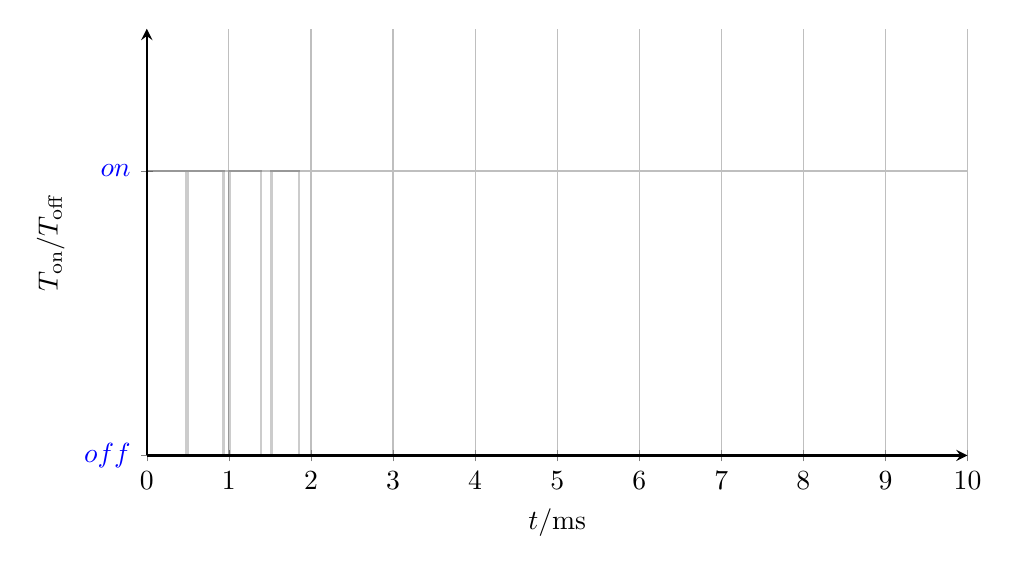
\begin{tikzpicture}
        \begin{axis}[
            xlabel={$t / \mathrm{ms}$},
            ylabel={$T_\mathrm{on}/T_\mathrm{off}$},
            axis lines=left,
            ymin=0, ymax=1.5,
            xmin=0, xmax=10,
            xtick={0,1,2,3,4,5,6,7,8,9,10},
            ytick={0,1},
            yticklabels={{\color{blue}$off$},{\color{blue}$on$}},
            thick,
            smooth,
            height=7cm,
            width=0.99\textwidth,
            grid
            ]
    
            
            \draw[opacity=0.2] 
                (axis cs:0, 1) -- (axis cs:0.48, 1) -- (axis cs:0.48, 0) -- (axis cs:0, 0) -- cycle;
            
            \draw[opacity=0.2] 
                (axis cs:0.5, 1) -- (axis cs:0.935, 1) -- (axis cs:0.935, 0) -- (axis cs:0.5, 0) -- cycle;
    
            
            \draw[opacity=0.2] 
                (axis cs:1.008, 1) -- (axis cs:1.388, 1) -- (axis cs:1.388, 0) -- (axis cs:1.008, 0) -- cycle;
    
            
            \draw[opacity=0.2] 
                (axis cs:1.52, 1) -- (axis cs:1.852, 1) -- (axis cs:1.852, 0) -- (axis cs:1.52, 0) -- cycle;

          %  \draw[opacity=0.2] 
            %    (axis cs:2,044, 1) -- (axis cs:1.852, 1) -- (axis cs:1.852, 0) -- (axis cs:1.52, 0) -- cycle;

                
    
        \end{axis}
    \end{tikzpicture}
    

    \caption{Test Caption}
    \label{fig:QuadraticFunction}
\end{figure}

\begin{solutionblock}
    \begin{equation}
        \frac{\mathrm{d}i'}{\mathrm{d}}  = \frac{1}{L} \hat U_\mathrm{1} \sin(\omega t)
    \end{equation}
   % \begin{equation}
    %    i' = \frac{1}{L \omega} \hat U_\mathrm{1} \[ \int_{0}^{T_\mathrm{p1_off}} \sin (\omega t) \,dt \]
   % \end{equation}
    
\end{solutionblock}

\subtask{Complete the current curve for a switching frequency $f_\mathrm{T2} = \SI{2}{\kilo\hertz}$ and a inductance $L = \SI{5}{\milli\henry}$ in \autoref{fig:Current i' control signal ex05}. Note: At the time $t =0$ is $i'=0$. The switch-on and switch-off times are determined by the control signal of the transistor $T$ and are summarized for the first 4 switching times in \autoref{tab:switching_times}.}

\begin{table}[ht]
    \centering
    
    \begin{tabular}{lcccc}
        \toprule
        & $i = 1$ & $2$ & $3$ & $4$ \\
        \midrule
        $T_{pi,OFF}$ & \SI{480}{\micro\second} & \SI{935}{\micro\second} & \SI{1388}{\micro\second} & \SI{1852}{\micro\second} \\
        $T_{pi,ON}$  & \SI{500}{\micro\second} & \SI{1008}{\micro\second} & \SI{1520}{\micro\second} & \SI{2044}{\micro\second} \\
        \bottomrule
    \end{tabular}
    \caption{Switching times $T_{pi,OFF}$ and $T_{pi,ON}$ for different $i$-Values.}
    \label{tab:switching_times}
\end{table}

\begin{figure}[htb]
    \centering
    % First TikZ picture
    \begin{tikzpicture}
        \begin{axis}[
            xlabel={$t / \mathrm{ms}$},
            ylabel={$u_\mathrm{1}(t) / u_\mathrm{1}(t)-400 / 400-u_\mathrm{1}(t) / \mathrm{V}$},
            axis lines=left,
            ymin=-400, ymax=400,
            xmin=0, xmax=10,
            xtick={0, 1, 2, 3, 4, 5, 6, 7, 8, 9, 10},
            ytick={-400, -300, -200, -100, 0, 100, 200, 300, 400},
            thick,
            smooth,
            no markers,
            height=7cm,
            width=0.99\textwidth,
            grid
            ]
            
            \addplot[domain=0:10, samples=200, thick, signalblue] 
            {-13.2 * (x - 5)^2 + 330};
            \addplot[domain=0:10, samples=200, thick, signalblue] 
            {-12.6 * (x - 5)^2 - 85};
            \addplot[domain=0:10, samples=200, thick, signalblue] 
            {12.8 * (x - 5)^2 + 80};
                      
            
            



            \draw[opacity=0.2] 
            (axis cs:0, 400) -- (axis cs:0.48, 400) -- (axis cs:0.48, -400) -- (axis cs:0, -400) -- cycle;

            \draw[opacity=0.2] 
                (axis cs:0.5, 400) -- (axis cs:0.935, 400) -- (axis cs:0.935, -400) -- (axis cs:0.5, -400) -- cycle;
    
            
            \draw[opacity=0.2] 
                (axis cs:1.008, 400) -- (axis cs:1.388, 400) -- (axis cs:1.388, -400) -- (axis cs:1.008, -400) -- cycle;
    
            
            \draw[opacity=0.2] 
                (axis cs:1.52, 400) -- (axis cs:1.852, 400) -- (axis cs:1.852, -400) -- (axis cs:1.52, -400) -- cycle;

        \end{axis}
    \end{tikzpicture} 

    \caption{Current curve $i'$ and $i'*$ and drive signal for the power transistor $T$}
    \label{fig:drive signal for the power transistor TH}
\end{figure}


\subtask{Approximately sketch the envelope of the current ripple in \autoref{fig:Current i' control signal ex05}. Sketch the voltage across the inductor in \autoref{fig:Voltage curve ul signal Transistor ex05} and enter the local average value of the voltage as an approximation. How would the switch-on/switch-off ratio of the transistor have to be changed before and after the current peak in order to bring the average actual current value closer to the current setpoint?}

\subtask{Calculate the losses in the diode $D_\mathrm{5}$.}

\subtask{Dimension the output capacitance $C$ in a way that the amplitude of the output voltage ripple is at twice the mains frequency $\Delta u_{\mathrm{2}}<0.05U_{\mathrm{2}}$.
Note: Take the approach using the instantaneous input power $p_{\mathrm{1}(t)}$ and assume that this power is fed directly to the output.}

\subtask{Calculate the RMS value of the current through the capacitor $I_{\mathrm{C}}$.
Note: The mean value of the current through the capacitor is $\overline i_{\mathrm{C}}=0$!}

\subtask{The current carrying capacity of the capacitor is $\frac{\SI{10}{\ampere}}{\SI{1}{\milli\farad}}$. How large must its capacitance be selected? Is the permissible output voltage fluctuation from 2.7 or is it the current carrying capacity that determines the capacitance?}

\subtask{What is the current load (effective and average value) of the mains diodes?}